\section{ArXe-Clusters}
In heteronuclear ArXe clusters \ac{ICD} and \ac{ETMD}3 are theoretically
possible after creation of an Ar3s vacancy. The final states of these processes
are characterized by Ar3p$^{-1}$Xe5p$^{-1}$ and Xe5p$^{-1}$Xe5p$^{-1}$,
respectively. As discussed in section \ref{section:icd_geom}, all \ac{ICD}
channels are closed
for distances shorther than \unit[10]{\AA}. From this perspective the
slower \ac{ETMD}3, which is energetically accessible at equilibrium geometries
of the ArXe$_2$ trimer should be
observable in experiment \cite{Fasshauer10}. 

In the following, first the basic cluster and spin-orbit coupling effects
are investigated using easiest model
structures. Afterwards, cluster structures investigated and compared to experiment.


\subsection{One Argon Atom on a Xenon Surface}
In order to model the decay processes in clusters a cutout of an cluster
is modelled by layers of xenon atoms in an \ac{fcc} structure. On these
layers, one argon atom is placed in either a \ac{fcc} or an \ac{hcp} position
as shown in Figure \ref{figure:model_clusters}. The atomic distances are
assumed to equal the sum of the corresponding van der Waals radii given in
Table \ref{table:vdWaalsradii}. The results of this section were published
in \cite{Fasshauer13}.

\begin{figure}[htb]
 \centering
 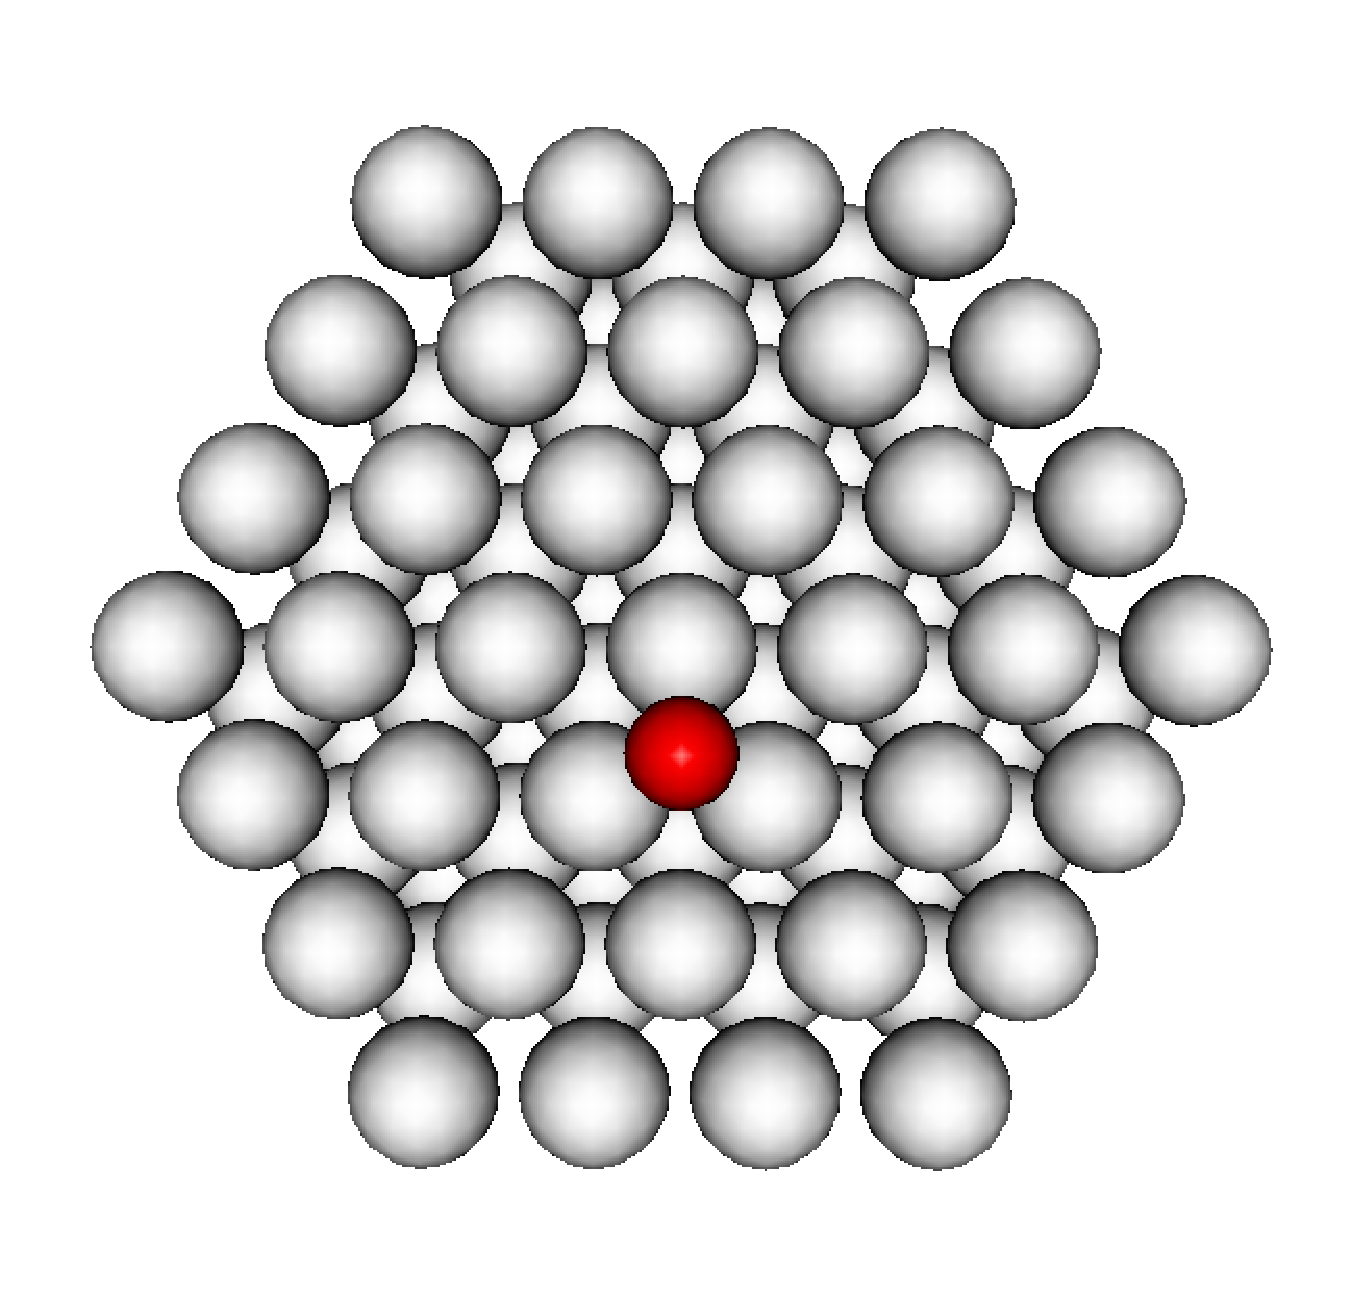
\includegraphics[scale=0.27]{pics/fcc.eps}
 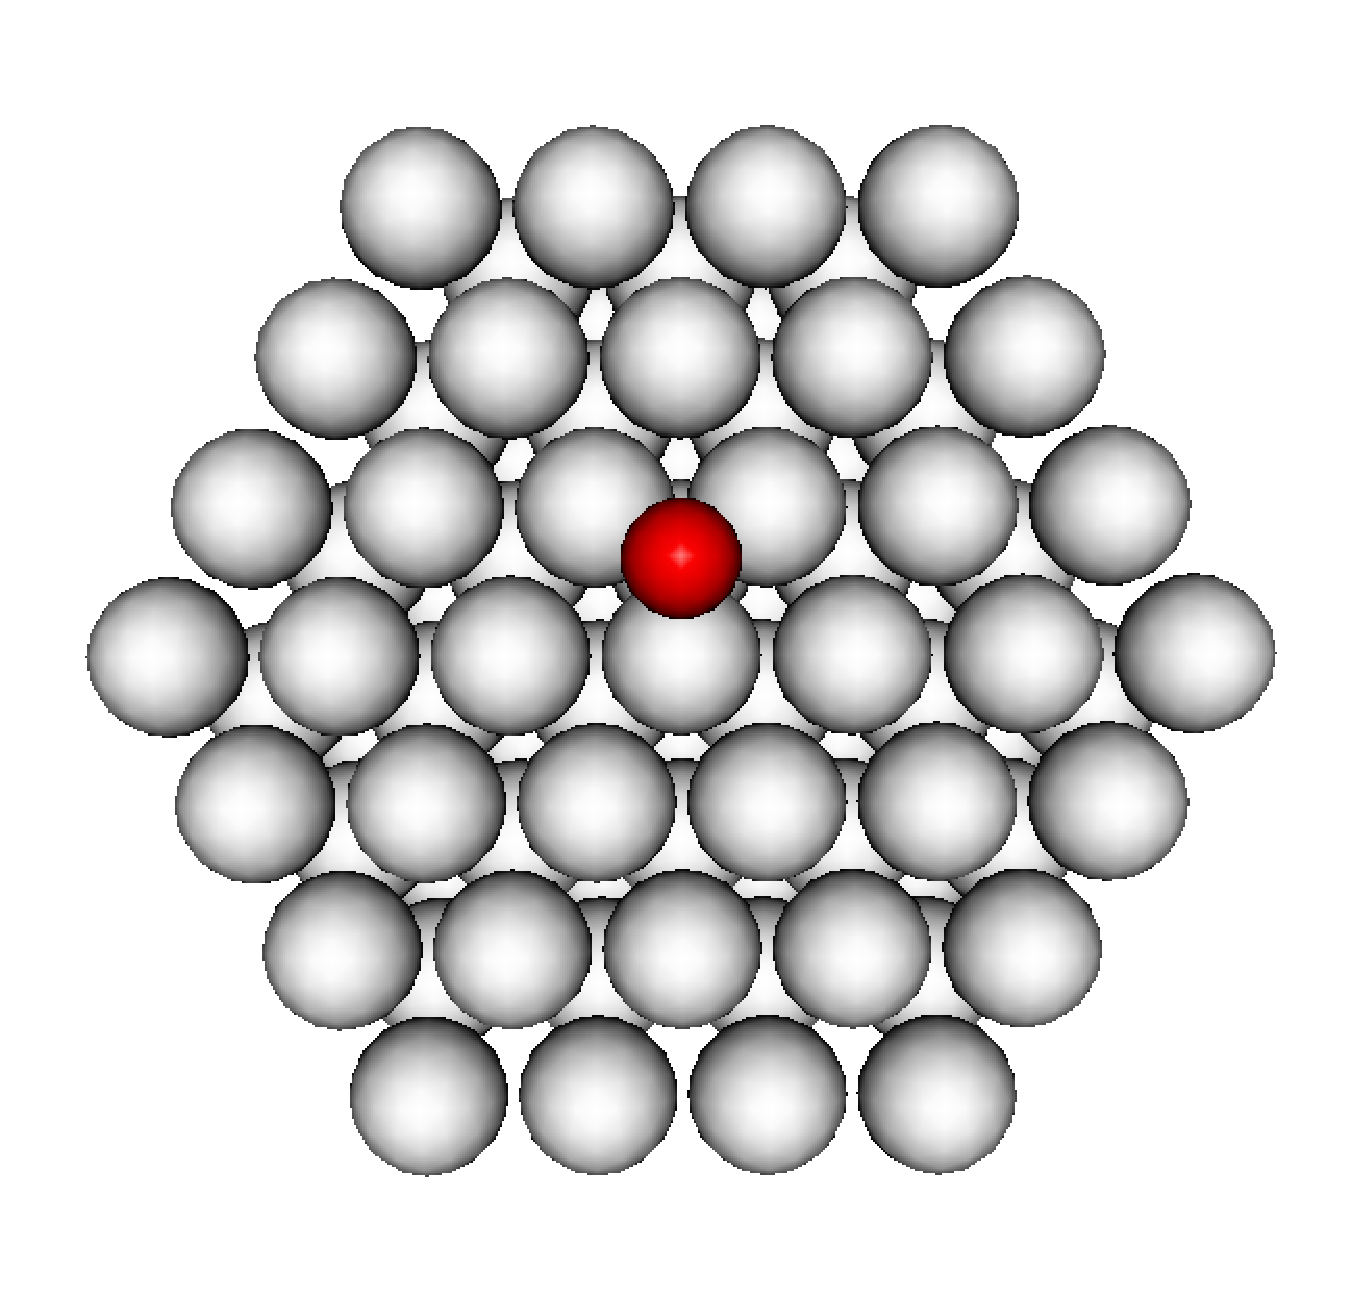
\includegraphics[scale=0.27]{pics/hcp.eps}
 \caption{Model structures of ArXe clusters.\\
          Left panel: Argon atom placed
          in an \ac{fcc} position on xenon atom layers in \ac{fcc} structure.\\
          Right panel: Argon atom placed
          in an \ac{hcp} position on xenon atom layers in \ac{hcp} structure.}
 \label{figure:model_clusters}
\end{figure}

%The initial and final state energies are estimated by shifted atomic
%ionization energies.
Since atoms in clusters interact with each other and especially
charges are stabilized in noble gas clusters, the atomic
ionization energies  in Table \ref{table:noble_atom_ionization} alone
are no good approximation. In order to take care of
this stabilization effect, the ionization energies are corrected by experimentally
observed shifts between atomic and cluster ionization energies of homonuclear
clusters given in Table
\ref{table:cluster_shifts} in the appendix. These shifts do not account for
higher or
lower charge stabilization by neighbouring atoms of other elements.

Achieved from these shifted ionization energies the potential curves of
initial and final states are shown in Figure \ref{ArXe_energy_curves_shifted}.

\begin{figure}[htb]
 \centering
 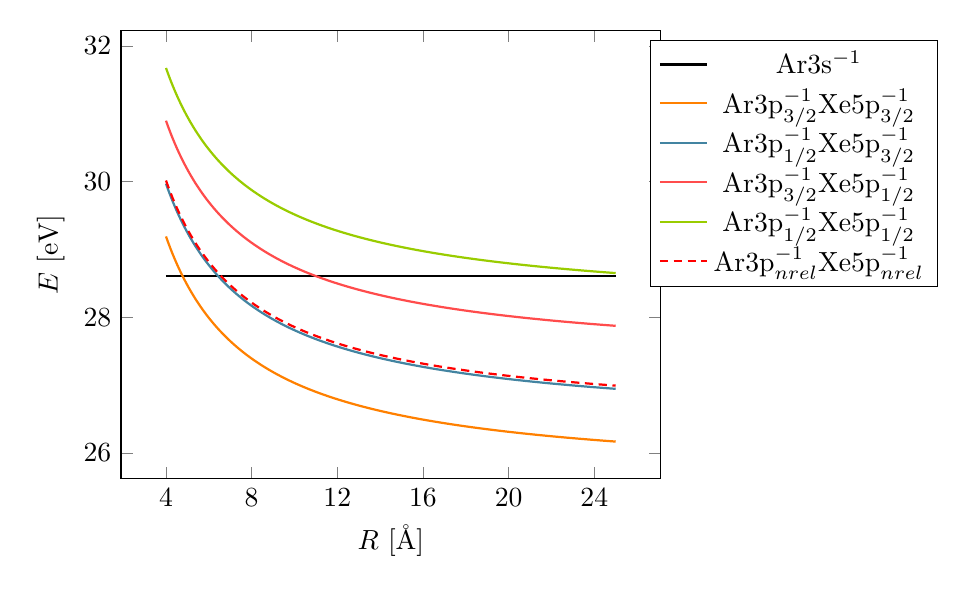
\begin{tikzpicture}
    \begin{axis}[domain=4.0:25,
                 samples = 200,
                 xtick={4.0,8.0,...,24},
                 %xticklabels={$-\pi$,$-\frac \pi 2$,0,$\frac \pi 2$,$\pi$},
                 cycle list name = exotic,
                 legend style={anchor= north west},
                 xlabel={$R$ [\AA]},
                 ylabel={$E$ [eV]}
                 ]
      \addplot+[
                mark = none,
                black,
                thick
               ]
               {29.239 - 0.636};
      \addlegendentry{Ar3s$^{-1}$};
      \addplot+[
                mark = none,
                thick
               ]
               {15.7596 - 1.0 + 12.1298 - 1.3 + 14.39964 / x};
      \addlegendentry{Ar3p$_{3/2}^{-1}$Xe5p$_{3/2}^{-1}$};
      \addplot+[
                mark = none,
                thick
               ]
               {15.9371 - 0.4 + 12.1298 -1.3 + 14.39964 / x};
      \addlegendentry{Ar3p$_{1/2}^{-1}$Xe5p$_{3/2}^{-1}$};
      \addplot+[
                mark = none,
                thick
               ]
               {15.7596 - 1.0 + 13.4363 -0.9 + 14.39964 / x};
      \addlegendentry{Ar3p$_{3/2}^{-1}$Xe5p$_{1/2}^{-1}$};
      \addplot+[
                mark = none,
                thick
               ]
               {15.9371 -0.4 + 13.4363 - 0.9 + 14.39964 / x};
      \addlegendentry{Ar3p$_{1/2}^{-1}$Xe5p$_{1/2}^{-1}$};
      \addplot+[
                mark = none,
                thick
               ]
               {15.8188 - 0.8 + 12.5653 - 1.17 + 14.39964 / x};
      \addlegendentry{Ar3p$_{nrel}^{-1}$Xe5p$_{nrel}^{-1}$};
      %\draw[] (axis cs:\pgfkeysvalueof{/pgfplots/xmin},29.239) -- (axis cs:\pgfkeysvalueof{/pgfplots/xmax},29.239);
    \end{axis}
\end{tikzpicture}

 \caption{Initial and final state energies of the ICD channels of ArXe in the
          model of pairs calculated from shifted atomic ionization energies.
          Both the four relativistic channels and
          the non-relativistic estimate are shown. From the distance on, where
          the final state energy is lower than the initial state energy, the
          decay channel is open.}
 \label{ArXe_energy_curves_shifted}
\end{figure}

Compared to the results using unshifted ionization energies of section
\ref{section:icd_geom} the
channel opening distances are shorter.
In detail, they are \unit[4.78]{\AA}, \unit[6.44]{\AA}, \unit[11.02]{\AA}
and \unit[27.19]{\AA} for the Ar3p$_{3/2}^{-1}$Xe5p$_{3/2}^{-1}$,
Ar3p$_{1/2}^{-1}$Xe5p$_{3/2}^{-1}$, Ar3p$_{3/2}^{-1}$Xe5p$_{1/2}^{-1}$ and
Ar3p$_{1/2}^{-1}$Xe5p$_{1/2}^{-1}$ channel, respectively. The channel
opening distance of the non-relativistic estimate is \unit[6.58]{\AA}.
This means that all \ac{ICD} channels are still closed at the equilibrium
distance of the ArXe dimer being \unit[4.04]{\AA}. But inside a
cluster also larger distances are
realized. Already for the next-nearest neighbours the
Ar3p$_{3/2}^{-1}$Xe5p$_{3/2}^{-1}$ channel is open. Hence, the \ac{ICD}
process can not be neglected in the further discussion.

The potential curves of the initial and final states of the \ac{ETMD}3
process are shown in Figure \ref{figure:ArXe_energy_etmd_curves}, where
$d$ denotes the distance between the two xenon atoms.

\begin{figure}[htb]
 \centering
 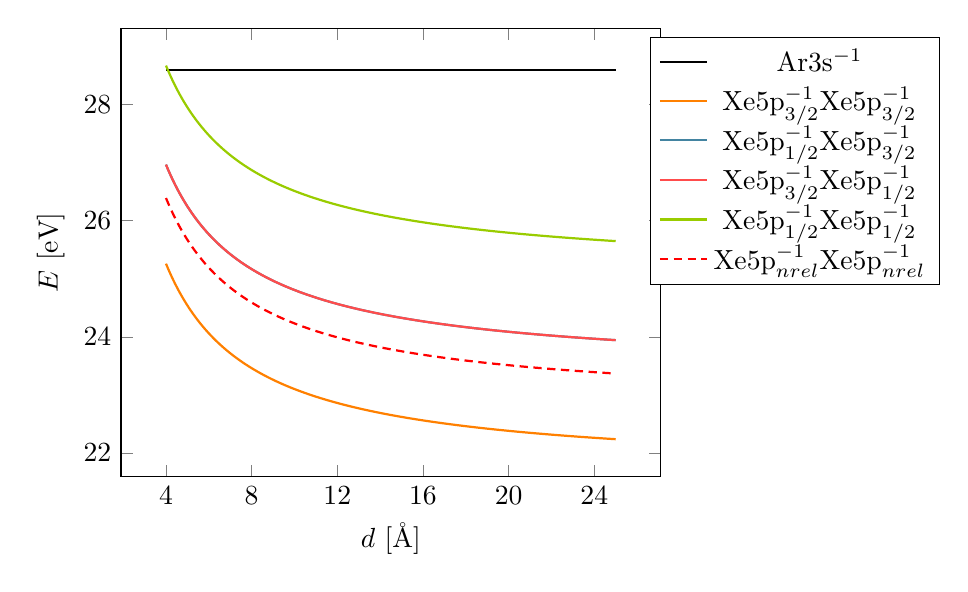
\begin{tikzpicture}
    \begin{axis}[domain=4.0:25,
                 samples = 200,
                 xtick={4.0,8.0,...,24},
                 %xticklabels={$-\pi$,$-\frac \pi 2$,0,$\frac \pi 2$,$\pi$},
                 cycle list name = exotic,
                 legend style={anchor= north west},
                 xlabel={$d$ [\AA]},
                 ylabel={$E$ [eV]}
                 ]
      \addplot+[
                mark = none,
                black,
                thick
               ]
               {29.239 - 0.636};
      \addlegendentry{Ar3s$^{-1}$};
      \addplot+[
                mark = none,
                thick
               ]
               {12.1298 - 1.3 + 12.1298 - 1.3 + 14.39964 / x};
      \addlegendentry{Xe5p$_{3/2}^{-1}$Xe5p$_{3/2}^{-1}$};
      \addplot+[
                mark = none,
                thick
               ]
               {13.4363 - 0.9 + 12.1298 -1.3 + 14.39964 / x};
      \addlegendentry{Xe5p$_{1/2}^{-1}$Xe5p$_{3/2}^{-1}$};
      \addplot+[
                mark = none,
                thick
               ]
               {12.1298 - 1.3 + 13.4363 -0.9 + 14.39964 / x};
      \addlegendentry{Xe5p$_{3/2}^{-1}$Xe5p$_{1/2}^{-1}$};
      \addplot+[
                mark = none,
                thick
               ]
               {13.4363 - 0.9 + 13.4363 - 0.9 + 14.39964 / x};
      \addlegendentry{Xe5p$_{1/2}^{-1}$Xe5p$_{1/2}^{-1}$};
      \addplot+[
                mark = none,
                thick
               ]
               {12.5653 - 1.17 + 12.5653 - 1.17 + 14.39964 / x};
      \addlegendentry{Xe5p$_{nrel}^{-1}$Xe5p$_{nrel}^{-1}$};

    \end{axis}
\end{tikzpicture}

 \caption{Initial and final state energies of the \ac{ETMD}3 channels
          in the model of triples calculated from shifted atomic ionization
          energies.}
 \label{figure:ArXe_energy_etmd_curves}
\end{figure}

In the applied model, the final state energies of the
Xe5p$_{1/2}^{-1}$Xe5p$_{3/2}^{-1}$ and
the Xe5p$_{3/2}^{-1}$Xe5p$_{1/2}^{-1}$ are degenerate, but the channels
differ by the quantum
numbers of the vacancy filling an the emitted electron. Hence, the decay
widths are not necessarily equal and need to be treated separately.
For all distances larger than the equilibrium distance of \unit[4.32]{\AA}
all \ac{ETMD}3 channels are open. Therefore, the decay can occur with
nearest neighbours, which enables the highest possible decay width.

From the consideration of channel opening distances alone, it is not clear, whether
one of the two competing processes is much faster and would hence dominate
an experimental spectrum. Another aspect of clusters is the multitude of
possible decay partners. For the \ac{ICD}, the number of decay partners equals
the number of xenon atoms $N_{Xe}$, while for the \ac{ETMD}3 process the number
of triples for each argon atoms is given by $N_{Xe}^2$. This means that
the \ac{ETMD}3 is statistically favoured above the \ac{ICD} in clusters with
xenon cores consisting of more than one xenon atom.

The decay widths of the \ac{ICD} and \ac{ETMD}3 process for the model
structures were calculated using the model of pairs and triples introduced in
chapter \ref{chapter:geom}. For this the model structures were decomposed
into all possible pairs and triples. For each pair and triple with an energy
transfer distance $R$ smaller than \unit[11]{\AA}, the decay width was evaluated
using
the asymptotic approximations of equations
(\ref{reltheolifetime_exp}) and (\ref{reltheolifetimeetmd_exp}) and the
experimentally obtained atomic properties of Tables
\ref{table:noble_atom_ionization}, \ref{table:noble_atom_properties} and
\ref{table:cluster_shifts}, and absolute ionization cross sections from reference
\cite{West78}. For the energy transfer distance $R$ of the \ac{ETMD}3 process
the reference point was chosen to be the center of mass of
$S_1$. 
Then, the decay widths of both model structures were combined normalized
to one initially ionized argon atom.

\begin{figure}[]
 \centering
 \begin{tikzpicture}[scale=1.0]

\begin{axis}[%scale=1.5,
             domain=0:7,
             restrict expr to domain={x}{0:7},
             %restrict expr to domain={y}{1.0E-12:7},
             xlabel={E [eV]},
             %xtick={30,50,...,170},
             %xticklabels={2,4,6,8,10,12,15,20,25},
             %ytick={-1.0,-0.8,...,1.0},
             %yticklabels={1.0,0.8,0.6,0.4,0.2,0.0,0.2,0.4,0.6,0.8,1.0},
             ylabel={$\Gamma$ [eV]},
             scale only axis,
             width=\textwidth-1.5cm,
             height=8cm,
             %ybar stacked
             ]

%ICD
\addplot+[ycomb,
         mark=.,
         very thick,
         diplom1,
         forget plot
        ]
        table[
        x expr = \thisrowno{0},
        y expr = \thisrowno{1}
        ]
        {data/arxe_model_icd_rel.dat};
        \addlegendimage{line legend, diplom1, very thick};
        \addlegendentry{ICD};

%ETMD
\addplot+[ycomb,
         mark=.,
         very thick,
         diplom2,
         forget plot
        ]
        table[
        x expr = \thisrowno{0},
        y expr = \thisrowno{1}
        ]
        {data/arxe_model_etmd_rel.dat};
        \addlegendimage{line legend, diplom2, very thick};
        \addlegendentry{ETMD};


%Folded
\addplot[
         mark=none,
         color=gray,
         dotted,
         thick
         ]
         table[
         x expr=\thisrowno{0},
         y expr=\thisrowno{1}
         ]
         {data/arxe_model_icd_rel.sp};
         \addlegendentry{ICD spectrum};

\addplot[
         mark=none,
         color=gray,
         dashed,
         thick
         ]
         table[
         x expr=\thisrowno{0},
         y expr=\thisrowno{1}
         ]
         {data/arxe_model_etmd_rel.sp};
         \addlegendentry{ETMD spectrum};

\addplot[
         mark=none,
         color=gray,
         thick
         ]
         table[
         x expr=\thisrowno{0},
         y expr=\thisrowno{1}
         ]
         {data/arxe_model_kombi_rel.sp};
         \addlegendentry{full spectrum};



\end{axis}
\end{tikzpicture}

 \begin{tikzpicture}[scale=1.0]

\begin{axis}[%scale=1.5,
             domain=0:7,
             restrict expr to domain={x}{0:7},
             %restrict expr to domain={y}{1.0E-12:7},
             xlabel={E [eV]},
             %xtick={30,50,...,170},
             %xticklabels={2,4,6,8,10,12,15,20,25},
             %ytick={-1.0,-0.8,...,1.0},
             %yticklabels={1.0,0.8,0.6,0.4,0.2,0.0,0.2,0.4,0.6,0.8,1.0},
             ylabel={$\Gamma$ [eV]},
             scale only axis,
             width=\textwidth-1.5cm,
             height=8cm,
             %ybar stacked
             ]

%ICD
\addplot+[ycomb,
         mark=.,
         very thick,
         diplom1,
         forget plot
        ]
        table[
        x expr = \thisrowno{0},
        y expr = \thisrowno{1}
        ]
        {data/arxe_model_icd_nrel.dat};
        \addlegendimage{line legend, diplom1, very thick};
        \addlegendentry{ICD};

%ETMD
\addplot+[ycomb,
         mark=.,
         very thick,
         diplom2,
         forget plot
        ]
        table[
        x expr = \thisrowno{0},
        y expr = \thisrowno{1}
        ]
        {data/arxe_model_etmd_nrel.dat};
        \addlegendimage{line legend, diplom2, very thick};
        \addlegendentry{ETMD};


%Folded
\addplot[
         mark=none,
         color=gray,
         dotted,
         thick
         ]
         table[
         x expr=\thisrowno{0},
         y expr=\thisrowno{1}
         ]
         {data/arxe_model_icd_nrel.sp};
         \addlegendentry{ICD spectrum};

\addplot[
         mark=none,
         color=gray,
         dashed,
         thick
         ]
         table[
         x expr=\thisrowno{0},
         y expr=\thisrowno{1}
         ]
         {data/arxe_model_etmd_nrel.sp};
         \addlegendentry{ETMD spectrum};

\addplot[
         mark=none,
         color=gray,
         thick
         ]
         table[
         x expr=\thisrowno{0},
         y expr=\thisrowno{1}
         ]
         {data/arxe_model_kombi_nrel.sp};
         \addlegendentry{full spectrum};



\end{axis}
\end{tikzpicture}

 \caption{\ac{ICD} and \ac{ETMD}3 secondary electron spectra for the model
          structures of Figure \ref{figure:model_clusters}. To guide the
          eye of the reader, the spectra
          were folded with Gaussians of \unit[300]{meV} and \unit[600]{meV}
          for the \ac{ICD} and \ac{ETMD}, respectively.\\
          Upper panel: Relativistic spectrum. Lower panel: Non-relativistic
          spectrum.}
 \label{figure:arxe_model}
\end{figure}

The resulting secondary electron spectra of the \ac{ICD} and
\ac{ETMD}3 processes are shown in Figure \ref{figure:arxe_model} for the
relativistic and the non-relativistic estimate.
It has to be kept in mind that the non-relativistic results intrinsically
incorporates scalar-relativistic effects in the experimentally obtained variables.

In the relativistic treatment (upper panel), the \ac{ETMD} causes three main
peaks at \unit[0.243]{eV}, \unit[1.950]{eV} and \unit[3.656]{eV}
corresponding to decay
processes involving nearest neighbours. The peak at \unit[3.343]{eV} stems
from the Xe5p$_{3/2}^{-1}$Xe5p$_{3/2}^{-1}$ channel, whereas the peak
at \unit[1.637]{eV} originates from the sum of the energetically degenerate
Xe5p$_{1/2}^{-1}$Xe5p$_{3/2}^{-1}$ and Xe5p$_{3/2}^{-1}$Xe5p$_{1/2}^{-1}$
channels. The Xe5p$_{1/2}^{-1}$Xe5p$_{1/2}^{-1}$ channel evokes the peak
at \unit[0.243]{eV}.
The \ac{ICD} process causes a multitude of smaller peaks at kinetic
energies of the emitted electron below \unit[1.8]{eV}. These originate from the
Ar3p$_{3/2}^{-1}$Xe5p$_{3/2}^{-1}$ and the Ar3p$_{1/2}^{-1}$Xe5p$_{3/2}^{-1}$
channels of pairs characterized by different distances.
The folded spectrum shows a large peak close to zero with two shoulders
caused by the \ac{ETMD}3 process.

In the non-relativistic treatment (lower panel), the secondary
electron spectrum shows only one main \ac{ETMD} peak at \unit[2.525]{eV}
corresponding to the Xe5p$^{-1}$Xe5p$^{-1}$ channel.
At energies \unit[<1.0]{eV} the \ac{ICD} peaks are shown. These correspond
to the Ar3p${-1}$Xe5p$^{-1}$ channel only and hence stem from pairs of
different distances.
The combined, folded spectrum shows two distinct peaks for the \ac{ICD} and
\ac{ETMD}3 process.

In order to guide the eye of the reader, the spectra were folded with
Gaussians of \unit[300]{meV} and \unit[600]{meV}
for the ICD and ETMD3, respectively. The broadening of the ICD peak due
to dynamics was estimated from the potential curve of the ArXe dimer. For
the ETMD3 the dynamics are by far more complex and since no reasonable
calculation was at hand, the broadening was estimated to be twice the width
of the ICD process.

The total calculated decay widths are shown in Table
\ref{table:arxe_widths_model}. From these numbers the spin-orbit coupled
reults are not equal to the results obtained in the non-relativistic estimate,
but similar. This can be explained by the multitude of channels, which
open at different distances and therefore, the basis of pairs and triples
included in the open channel calculations differ. In both the relativistic and
the non-relativistic treatment,
the decay width of the \ac{ICD} is slightly larger than the one of the
\ac{ETMD}3 process. Since all lifetimes are three orders of magnitude smaller
than the radiative lifetime of the Ar3s vacancy of \unit[4.684]{ns},
these processes outrule the radiative decay.
Because of the comparable decay widths of \ac{ICD} and \ac{ETMD}3, both
processes should be experimentally observable.

\begin{table}[bt]
 \centering
 \caption{Decay widths of the ICD and ETMD processes of the model structures.}
 \begin{tabular}{lcccc}
  \toprule
          & \multicolumn{2}{c}{$\Gamma$ [eV]} & \multicolumn{2}{c}{$\tau$ [ps]}\\
          & rel.               & nrel.              & rel. & nrel. \\
  \midrule
   ICD    & $8.3\cdot 10^{-4}$ & $9.2\cdot 10^{-4}$ & 0.79 & 0.71\\
   ETMD   & $7.2\cdot 10^{-4}$ & $5.6\cdot 10^{-4}$ & 0.92 & 1.18\\
   total  & $15.5\cdot 10^{-4}$& $14.8\cdot 10^{-4}$& 0.43 & 0.44\\
  \bottomrule
 \end{tabular}
 \label{table:arxe_widths_model}
\end{table}

\subsubsection{Conclusions}
The above discussion embarked on the investigation and calculation of electron
emission spectra of mixed ArXe clusters produced in electronic decay reactions
following ionization of inner-valence electrons of Ar.
Together with a suiTable cluster model and including
energy shifts due to the environment as well as statistical effects,
individual and total electron emission spectra were generated. Due to the
presence of xenon, spin-orbit coupling was shown to play a major role for an
adequate description of energies, ICD and ETMD thresholds and total lifetimes
of the individual processes and can not be neglected. The  relativistic
calculations of the ICD spectrum show that the ICD electrons are expected to
have kinetic energies below \unit[2]{eV}. The corresponding ETMD peak is
centered at \unit[2]{eV} and exhibits pronounced overlap with the ICD feature.
These results are in stark contrast to the non-relativistic total spectrum
exhibiting two well separated structures. In the relativistic formulation,
the ratio of the ETMD to ICD intensity is determined to be 0.87 underlying the
importance of both decay processes in ArXe clusters.
If several Ar layers surround the core of xenon atoms,
this ratio is expected to decrease.
This is due to the fact that ICD, an energy-transfer process, can happen
anywhere in the bulk, while ETMD involves electron transfer and, therefore,
proceeds exclusively at the argon-xenon interface. It should be noted that
experimental peak positions and intensities can be slightly different due to
a number of approximations inherent in the model such as the choice of initial
and final state energies, a fixed geometry and
the exclusion of dynamical processes.



\subsection{Cluster Structures}
In the following section, decay widths for complete shell cluster structures
of \ac{fcc} and icosahedral structure are investigated. The structures were
obtained from the scripts \verb|icoclus| and \verb|fccclus| described in
the appendix \ref{icoclus} and \ref{fccclus}.

\subsubsection{Dependence on Cluster Size and Number of Argon Layers}
Consider a xenon cluster described by a complete icosahedral or dodecahedral
structure with one additional layer of argon. With increasing cluster size,
the \emph{surface-to-bulk} ratio decreases. Both the \ac{ICD} and \ac{ETMD}
are interface
effects and hence the decay widths per ionized argon atom can be expected
to increase and finally
to converge to some value. However, for an \ac{ETMD} the electron donor atom
needs to be in immediate vicinity in order to have a significant decay
width. Therefore, the decay width increase of the two processes with increasing
cluster size can be expected to be different.

Additionally for a fixed xenon core size, different numbers of surrounding
complete shells of argon atoms are possible. Since the \ac{ETMD} is a pure
interface effect, its decay width per initially ionized atom can be expected to
decrease with an increasing number of argon shells. The same behaviour
is expected for the \ac{ICD} process. However, since the process is also
able to occur with next-nearest neighbours, the decrease of the decay width
is expected to be less pronounced.

\begin{table}
 \centering
 \caption{ICD and ETMD decay widths in eV for ArXe icosahedral clusters with
          increasing core cluster size and 1 -- 4 layers of argon.
          In the last part the percentage of ETMD compared to the
          total decay is given.}
 %\small
 \begin{tabular}{clcccc}
  \toprule
   &  $c_{core}$ & 1 layer     & 2 layers             & 3 layers             & 4 layers \\
  \midrule
   \multirow{5}{*}{\rotatebox[origin=c]{90}{ICD}}  
   & 2 & 1.880$\cdot 10^{-4}$ & 1.336$\cdot 10^{-4}$ & 7.211$\cdot 10^{-5}$ & 4.220$\cdot 10^{-5}$  \\
   & 3 & 3.207$\cdot 10^{-4}$ & 2.219$\cdot 10^{-4}$ & 1.299$\cdot 10^{-4}$ & 8.117$\cdot 10^{-5}$  \\
   & 4 & 4.004$\cdot 10^{-4}$ & 2.812$\cdot 10^{-4}$ & 1.733$\cdot 10^{-4}$ & 1.132$\cdot 10^{-4}$  \\
   & 5 & 4.522$\cdot 10^{-4}$ & 3.230$\cdot 10^{-4}$ & 2.060$\cdot 10^{-4}$ & 1.388$\cdot 10^{-4}$  \\
   & 6 & 4.879$\cdot 10^{-4}$ & 3.536$\cdot 10^{-4}$ & 2.311$\cdot 10^{-4}$ & 1.592$\cdot 10^{-4}$  \\
  \midrule
   \multirow{5}{*}{\rotatebox[origin=c]{90}{ETMD3}}  
   & 2  &  1.187$\cdot 10^{-4}$  &  3.722$\cdot 10^{-5}$  &   1.685$\cdot 10^{-5}$  &  9.101$\cdot 10^{-6}$  \\
   & 3  &  1.969$\cdot 10^{-4}$  &  7.133$\cdot 10^{-5}$  &   3.581$\cdot 10^{-5}$  &  2.087$\cdot 10^{-5}$  \\
   & 4  &  2.429$\cdot 10^{-4}$  &  9.507$\cdot 10^{-5}$  &   5.072$\cdot 10^{-5}$  &  3.104$\cdot 10^{-5}$  \\
   & 5  &  2.726$\cdot 10^{-4}$  &  1.119$\cdot 10^{-4}$  &   6.210$\cdot 10^{-5}$  &  3.929$\cdot 10^{-5}$  \\
   & 6  &  2.931$\cdot 10^{-4}$  &  1.242$\cdot 10^{-4}$  &   7.092$\cdot 10^{-5}$  &  4.597$\cdot 10^{-5}$  \\
  \midrule
   \multirow{5}{*}{\rotatebox[origin=c]{90}{\% ETMD3}}  
   & 2  &   38.71  &  21.79  &  18.94  &  17.74  \\
   & 3  &   38.05  &  24.32  &  21.60  &  20.45  \\
   & 4  &   37.76  &  25.27  &  22.64  &  21.52  \\
   & 5  &   37.61  &  25.72  &  23.16  &  22.07  \\
   & 6  &   37.53  &  26.00  &  23.48  &  22.41  \\
  \bottomrule
 \end{tabular}
 \label{table:ico_size}
\end{table}


\begin{table}
 \centering
 \caption{ICD and ETMD decay widths in eV for ArXe dodecahedral clusters with
          increasing core cluster size and 1 -- 3 layers of argon.
          In the last part the percentage of ETMD compared to the
          total decay is given.}
 %\small
 \begin{tabular}{clccc}
  \toprule
   &  $c_{core}$ & 1 layer     & 2 layers             & 3 layers          \\%   & 4 layers \\
  \midrule
   \multirow{5}{*}{\rotatebox[origin=c]{90}{ICD}}  
   & 2 &  1.856$\cdot 10^{-4}$  & 1.437$\cdot 10^{-4}$  &  7.877$\cdot 10^{-5}$ \\ % &  4.645$\cdot 10^{-5}$    \\
   & 3 &  3.327$\cdot 10^{-4}$  & 2.418$\cdot 10^{-4}$  &  1.434$\cdot 10^{-4}$ \\ % &  9.023$\cdot 10^{-5}$    \\
   & 4 &  4.227$\cdot 10^{-4}$  & 3.099$\cdot 10^{-4}$  &  1.933$\cdot 10^{-4}$ \\ % &  1.270$\cdot 10^{-4}$    \\
   & 5 &  4.815$\cdot 10^{-4}$  & 3.579$\cdot 10^{-4}$  &  2.309$\cdot 10^{-4}$ \\ % &  1.565$\cdot 10^{-4}$    \\
   & 6 &  5.226$\cdot 10^{-4}$  & 3.931$\cdot 10^{-4}$  &  2.597$\cdot 10^{-4}$ \\ % &  1.800$\cdot 10^{-4}$    \\
  \midrule
   \multirow{5}{*}{\rotatebox[origin=c]{90}{ETMD}}  
   & 2 &  1.727$\cdot 10^{-4}$ & 5.416$\cdot 10^{-5}$ &  2.452$\cdot 10^{-5}$ \\ % &  1.324$\cdot 10^{-5}$      \\
   & 3 &  2.738$\cdot 10^{-4}$ & 9.920$\cdot 10^{-5}$ &  4.979$\cdot 10^{-5}$ \\ % &  2.903$\cdot 10^{-5}$      \\
   & 4 &  3.318$\cdot 10^{-4}$ & 1.299$\cdot 10^{-4}$ &  6.928$\cdot 10^{-5}$ \\ % &  3.442$\cdot 10^{-5}$      \\
   & 5 &  3.687$\cdot 10^{-4}$ & 1.514$\cdot 10^{-4}$ &  8.403$\cdot 10^{-5}$ \\ % &  5.317$\cdot 10^{-5}$      \\
   & 6 &  3.941$\cdot 10^{-4}$ & 1.671$\cdot 10^{-4}$ &  9.539$\cdot 10^{-5}$ \\ % &  6.183$\cdot 10^{-5}$      \\
  \midrule
   \multirow{5}{*}{\rotatebox[origin=c]{90}{\% ETMD}}  
   & 2 &  48.20 &    27.37 &   23.74 \\ %&     22.19  \\
   & 3 &  45.14 &    29.09 &   25.77 \\ %&     24.34  \\
   & 4 &  43.98 &    29.53 &   26.39 \\ %&            \\
   & 5 &  43.37 &    29.72 &   26.68 \\ %&     25.36  \\
   & 6 &  42.99 &    29.83 &   26.86 \\ %&     25.57  \\
  \bottomrule
 \end{tabular}
 \label{table:fcc_size}
\end{table}

These two hypotheses are tested in this chapter for xenon core sizes
with $c= 2-6$ and 1 -- 4/3 additional layers of argon atoms around it for
both icosahedral and dodecahedral clusters.
The calculations were performed using the programme \verb|HARDRoC|
\cite{HARDRoC} and the same atomic data as in the preceding section
given in Tables \ref{table:noble_atom_ionization},
\ref{table:noble_atom_properties} and \ref{table:cluster_shifts}.
Here, in contrast to the previous model structures, the argon atom
is chosen as the reference point for the energy
transfer distance $R$ of the ETMD3.

The results are shown in Tables \ref{table:ico_size} and \ref{table:fcc_size}
for the icosahedral and dodecahedral clusters, respectively.
From this data the expected trend of increasing decay width with
increasing cluster size for both \ac{ICD} and \ac{ETMD} processes and
icosahedral and dodecahedral structures proven. The same holds for
the decrease of the decay width per argon atom and the contribution of the \ac{ETMD}
process to the total decay with increasing number
of surrounding argon layers.
However, the contribution of the \ac{ETMD} to the total decay with increasing
xenon core size is unexpected on first sight. For one layer of argon atoms
the ETMD contribution decreases with increasing cluster size, while it
increases for more argon layers. Here, two contrarian effects play a role.
On the one hand, the number of xenon atoms in the interface shell increases
compared to the number of argon atoms in the interface layer. This statistically
prefers the ETMD over the ICD. On the other hand for small xenon cores not all
ICD channels are open for most of the pairs. With increasing cluster size for some
atom pairs additional channels will be open compared to the smaller clusters.
This favours the ICD over the ETMD, where all channels are open for each
possible triple. The latter effect is most pronounced for small clusters as
well as for argon atoms in the interface region and
therefore, it dominates the trend for one layer of argon atoms, whereas for more
argon layers the statistical effects benefit the ETMD over the ICD.

Comparing the absolute decay width values for the icosahedral and dodecahedral
cluster structures it can be seen that the ICD decay widths are comparable
for both skeletal structures and that the ETMD decay widths of the dodecahedral
structures are larger than of the icosahedral structures. Hence, also the
ETMD contribution to the total decay width is higher for the dodecahedral
structures.
This feature can be explained by the different surfaces of the icosahedral
and dodecahedral (fcc) clusters. Both clusters have triangular surfaces.
However, the dodecahedral cluster has less triangular surfaces than the
icosahedral cluster and instead some square surfaces. In the latter, the
interatomic distances of argon and xenon atoms differ slightly
from the interatomic distances for argon atoms positioned on triangular surfaces.
Additionally, the number of triples significantly contributing to the
decay width is higher than on the triangular surfaces.
Therefore, the ETMD decay widths are larger
in dodecahedral clusters than in icosahedral clusters.
% by the distance of the next-nearest neighbours
%in these cluster structures. In icosahedral clusters the atomic distance
%within a shell is small compared to the interatomic distance of atoms
%of different shells, while the shortest interatomic distance
%in dodecahedral clusters
%is constant for atoms of the same and different shells. In case of the icosahedral
%clusters the atoms of the next shell do not contribute significantly, while
%they do for dodecahedral clusters. Therefore, the ETMD decay widths are larger
%in dodecahedral clusters than in icosahedral clusters.



\subsubsection{Modelling Experimental Spectra}

The secondary electron spectra of three ArXe cluster ensembles were measured by
Förstel and Hergenhahn in 2012 (see Figure \ref{figure:arxe_exp}).
They had mean xenon core sizes
of $\le100$, $\le300$ and $\le2057$ atoms. The number of additional argon
layers is unknown.
For the same experimental conditions the single ionization spectra were
measured. Therefore, the results given in Table \ref{table:exp_arxe_ionization}
are going to be used for the modelling of the secondary electron spectra.
It has to be noted that these numbers are average values of very broad
distributions.

\begin{figure}
 \centering
 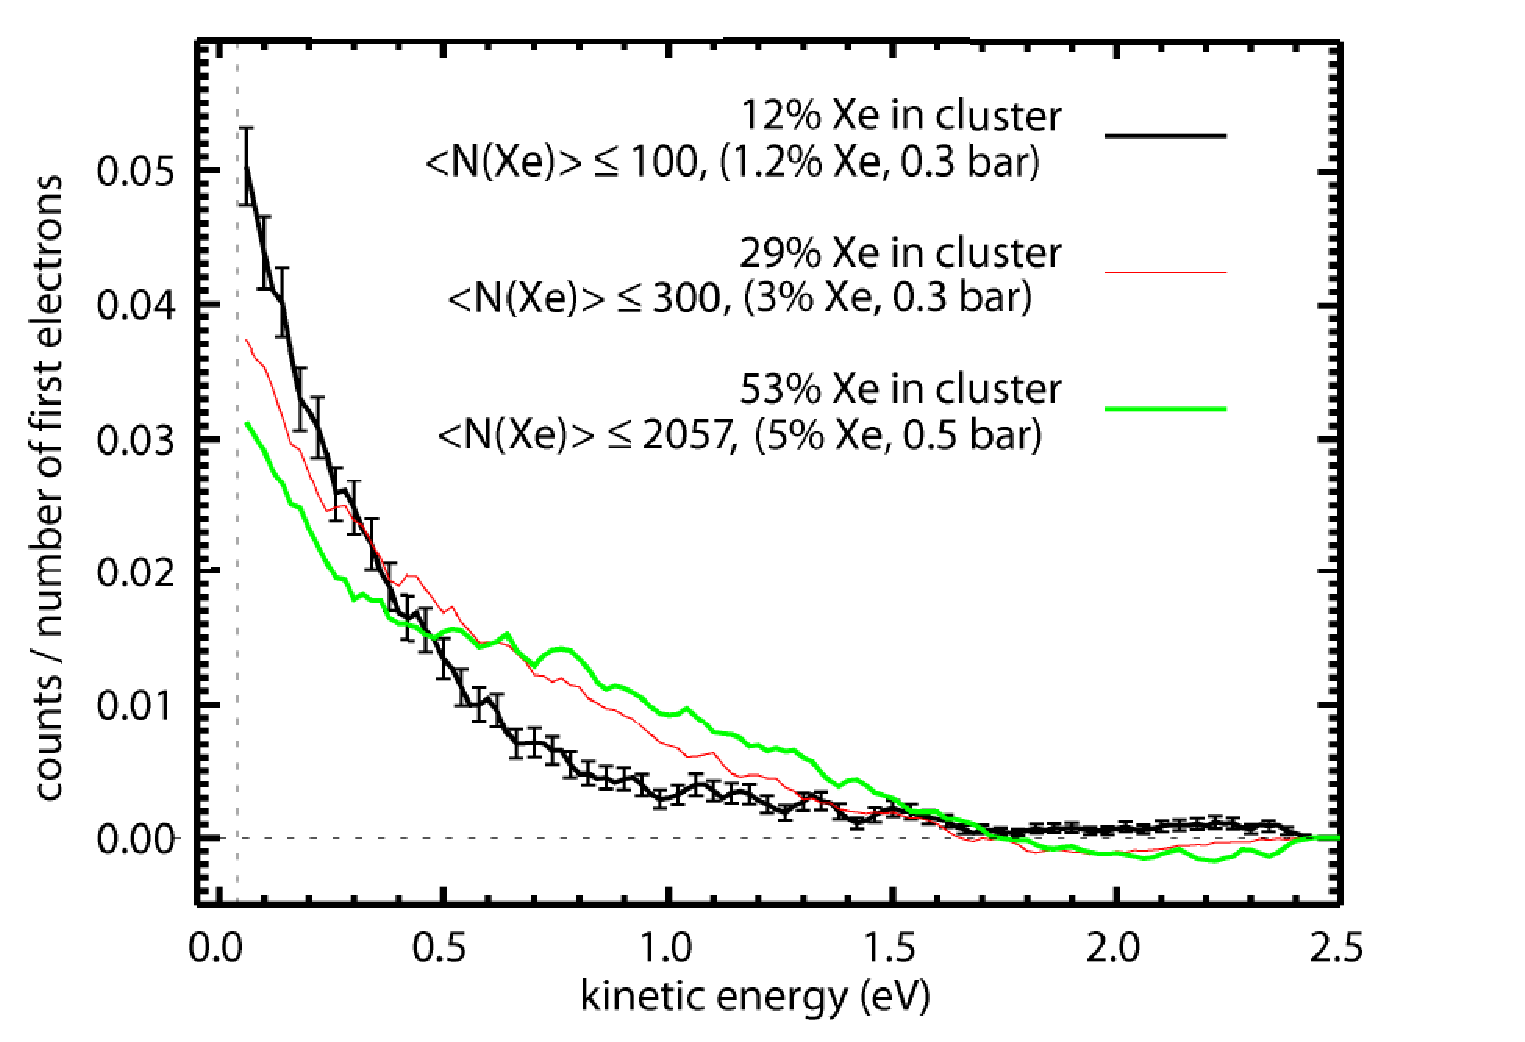
\includegraphics[scale=0.5]{pics/arxe_cluster_exp_groessenvergleich.eps}
 \caption{Experimental secondary electron spectra of different ArXe
          cluster ensembles.}
 \label{figure:arxe_exp}
\end{figure}

\begin{table}
 \centering
 \caption{Experimental ionization energies inside the ArXe clusters
          \cite{Foerstel_private}. These ionization energies are the
          average values of broad distributions.}
 \begin{tabular}{lcc}
  \toprule
             & SIP [eV]  & FWHM [eV] \\
  \midrule
   Xe5p$_{3/2}$ & 11.5   & 1.20 \\
   Xe5p$_{1/2}$ & 13.0   & 0.40 \\
   Ar3p         & 15.3   & 0.60 \\
   Ar3s         & 28.7   & 0.35 \\
  \bottomrule
 \end{tabular}
 \label{table:exp_arxe_ionization}
\end{table}

In the following the two larger cluster ensembles are going to be modelled
by cluster structures characterized by a 309 and 923 xenon atom core surrounded
by one additional layer of argon atoms. The latter was chosen, because the
calculations evaluating the ETMD decay width were computationally
too expensive for a xenon core of 2057 atoms in the current implementation.
The cluster with a 309 xenon atoms core can be expected to have an icosahedral
structure, while the larger cluster might be of dodecahedral shape. Therefore,
in the latter case both the fcc and the icosahedral structure are investigated.

The calculated spectrum of the 309 atom icosahedral model cluster is
shown in Figure \ref{figure:exp_309ico_arxe}. The spectra of the different
channels are plotted independently and the peak heights are not added.

\begin{figure}[t]
 \centering
 \begin{tikzpicture}[scale=1.0]

\begin{axis}[%scale=1.5,
             domain=0:7,
             restrict expr to domain={x}{0:7},
             %restrict expr to domain={y}{1.0E-12:7},
             xlabel={E [eV]},
             %xtick={30,50,...,170},
             %xticklabels={2,4,6,8,10,12,15,20,25},
             %ytick={-1.0,-0.8,...,1.0},
             %yticklabels={1.0,0.8,0.6,0.4,0.2,0.0,0.2,0.4,0.6,0.8,1.0},
             ylabel={$\Gamma$ [eV]},
             scale only axis,
             width=\textwidth-1.5cm,
             height=8cm,
             %ybar stacked
             ]

%ICD
\addplot+[ycomb,
         mark=.,
         very thick,
         Green,
         forget plot
        ]
        table[
        x expr = \thisrowno{0},
        y expr = \thisrowno{4}
        ]
        {data/exp_309ico_icd_arxe.dat};
        \addlegendimage{line legend, Green, very thick};
        \addlegendentry{Ar$_{3/2}$ Xe$_{3/2}$};

\addplot+[ycomb,
         mark=.,
         very thick,
         Goldenrod,
         forget plot
        ]
        table[
        x expr = \thisrowno{0},
        y expr = \thisrowno{2}
        ]
        {data/exp_309ico_icd_arxe.dat};
        \addlegendimage{line legend, Goldenrod, very thick};
        \addlegendentry{Ar$_{1/2}$ Xe$_{3/2}$};

\addplot+[ycomb,
         mark=.,
         very thick,
         LimeGreen,
         forget plot
        ]
        table[
        x expr = \thisrowno{0},
        y expr = \thisrowno{3}
        ]
        {data/exp_309ico_icd_arxe.dat};
        \addlegendimage{line legend, LimeGreen, very thick};
        \addlegendentry{Ar$_{3/2}$ Xe$_{1/2}$};

\addplot+[ycomb,
         mark=.,
         very thick,
         Fuchsia,
         forget plot
        ]
        table[
        x expr = \thisrowno{0},
        y expr = \thisrowno{1}
        ]
        {data/exp_309ico_icd_arxe.dat};
        \addlegendimage{line legend, Fuchsia, very thick};
        \addlegendentry{Ar$_{1/2}$ Xe$_{1/2}$};

%ETMD
\addplot+[ycomb,
         mark=.,
         very thick,
         diplom1,
         forget plot
        ]
        table[
        x expr = \thisrowno{0},
        y expr = \thisrowno{4}
        ]
        {data/exp_309ico_etmd_arxe.dat};
        \addlegendimage{line legend, diplom1, very thick};
        \addlegendentry{Xe$_{3/2}$ Xe$_{3/2}$};

\addplot+[ycomb,
         mark=.,
         very thick,
         orange,
         forget plot
        ]
        table[
        x expr = \thisrowno{0},
        y expr = \thisrowno{2}
        ]
        {data/exp_309ico_etmd_arxe.dat};
        \addlegendimage{line legend, orange, very thick};
        \addlegendentry{Xe$_{1/2}$ Xe$_{3/2}$};

\addplot+[ycomb,
         mark=.,
         very thick,
         diplom2,
         forget plot
        ]
        table[
        x expr = \thisrowno{0},
        y expr = \thisrowno{3}
        ]
        {data/exp_309ico_etmd_arxe.dat};
        \addlegendimage{line legend, diplom2, very thick};
        \addlegendentry{Xe$_{3/2}$ Xe$_{1/2}$};

\addplot+[ycomb,
         mark=.,
         very thick,
         diplom3,
         forget plot
        ]
        table[
        x expr = \thisrowno{0},
        y expr = \thisrowno{1}
        ]
        {data/exp_309ico_etmd_arxe.dat};
        \addlegendimage{line legend, diplom3, very thick};
        \addlegendentry{Xe$_{1/2}$ Xe$_{1/2}$};

%Folded
\addplot[
         mark=none,
         color=gray,
         dotted
         ]
         table[
         x expr=\thisrowno{0},
         y expr=\thisrowno{1}
         ]
         {data/exp_309ico_icd_arxe_spec.dat};
         \addlegendentry{ICD spectrum};

\addplot[
         mark=none,
         color=gray,
         dashed
         ]
         table[
         x expr=\thisrowno{0},
         y expr=\thisrowno{1}
         ]
         {data/exp_309ico_etmd_arxe_spec.dat};
         \addlegendentry{ETMD spectrum};

\addplot[
         mark=none,
         color=gray,
         ]
         table[
         x expr=\thisrowno{0},
         y expr=\thisrowno{1}
         ]
         {data/exp_309ico_kombi_arxe_spec.dat};
         \addlegendentry{full spectrum};


%\fill [red] (axis cs:0,1.1E-4) rectangle (axis cs:0.5,1.3E-4);

\end{axis}
\end{tikzpicture}

 \caption{Calculated secondary electron spectrum of the icosahedral
          309 xenon core cluster with one additional layer of argon
          atoms. Due to usage of experimental ionization energies of
          mixed clusters the peaks are shifted to lower energies compared
          to the spectra in Figure \ref{figure:arxe_model}.}
 \label{figure:exp_309ico_arxe}
\end{figure}

Compared to the spectra of the principle models in Figure \ref{figure:arxe_model},
the peak positions are shifted to lower kinetic energies of the emitted
electron by $\approx$\unit[1]{eV}. This at the same time leads to
channel closings especially for
the \ac{ICD}. Therefore, the spectrum is dominated by the \ac{ETMD} process.


%%%%%%%%%%%%%%%%%%%%%%%%%%%%%%%%%%%%
The secondary electron spectra for the large cluster with a xenon
core consisting of 923 atoms are shown in Figure \ref{figure:exp_923_arxe}.
In the upper panel, the spectrum of the icosahedral cluster is displayed.
As shown in the previous section, the increased number of bulk atoms
leads to ICD channel openings. Therefore, the ICD peak is more pronounced
than for the smaller cluster.

The spectrum of the dodecahedral cluster shape of fcc structure is shown in
the lower panel of Figure \ref{figure:exp_923_arxe}. As already qualitatively
discussed in the preceding section, also next-nearest neighbours can
significantly contribute to the total ETMD decay width. This property is
not observed in the easiest model structures,
because those model structures are only capable of modelling the behaviour of an
argon atom on a triangular and not a square surface.

Overall, the ICD dominates the secondary electron spectrum. However, this
is caused by the ICD peaks being centered at around \unit[0.5]{eV}, while
the ETMD peaks are spread over a large energy range. Additionally, dynamic
effects are expected to have a larger impact on the ETMD spectra with three
involved atoms than in the ICD spectra, which leads to an additional
broadening estimated in the folding of the spetra.




Since the ionization energies used for the modelling are mean values, they
might not represent the involved atoms correctly. The argon atoms with the
largest contributions to the ICD and ETMD decays are the atoms at the interface
region. However, it is not evident that the core is surrounded by one argon
layer only. Vacancies in the interface argon atoms might due to
their interaction with the
neighbouring xenon atoms be better stabilized than the average argon atom in the
cluster in case of several layers. Additionally, vacancies in the interface
xenon atoms might be less stabilized than in the average xenon atom.
Lower ionization energies of the Ar3s initial state would shift the spectrum
to lower kinetic energies, while lower ionization energies of the Ar3p
would shift the \ac{ICD} spectrum to higher kinetic energies.
Higher ionization energies of the Xe5p region would shift both the ICD and
the ETMD spectra to lower kinetic energies. Hereby, the ETMD spectrum would
have a larger shift. These contrary trends make it impossible to determine the
accurate peak positions for the clusters without extensive ionization energy
studies for different atomic positions inside the clusters.
Comparison to the experimental spectrum in Figure \ref{figure:arxe_exp}
suggests a shift to lower kinetic energies.
This might also be achieved by shorted interatomic distances in the cluster,
which might be caused by dynamical rearrangements of the atoms due to
the introduced vacancy.


\begin{figure}[]
 \centering
 \begin{tikzpicture}[scale=1.0]

\begin{axis}[%scale=1.5,
             domain=0:7,
             restrict expr to domain={x}{0:7},
             %restrict expr to domain={y}{1.0E-12:7},
             xlabel={E [eV]},
             %xtick={30,50,...,170},
             %xticklabels={2,4,6,8,10,12,15,20,25},
             %ytick={-1.0,-0.8,...,1.0},
             %yticklabels={1.0,0.8,0.6,0.4,0.2,0.0,0.2,0.4,0.6,0.8,1.0},
             ylabel={$\Gamma$ [eV]},
             scale only axis,
             width=\textwidth-1.5cm,
             height=8cm,
             %ybar stacked
             ]

%ICD
\addplot+[ycomb,
         mark=.,
         very thick,
         Green,
         forget plot
        ]
        table[
        x expr = \thisrowno{0},
        y expr = \thisrowno{4}
        ]
        {data/exp_923ico_icd_arxe.dat};
        \addlegendimage{line legend, Green, very thick};
        \addlegendentry{Ar$_{3/2}$ Xe$_{3/2}$};

\addplot+[ycomb,
         mark=.,
         very thick,
         Goldenrod,
         forget plot
        ]
        table[
        x expr = \thisrowno{0},
        y expr = \thisrowno{2}
        ]
        {data/exp_923ico_icd_arxe.dat};
        \addlegendimage{line legend, Goldenrod, very thick};
        \addlegendentry{Ar$_{1/2}$ Xe$_{3/2}$};

\addplot+[ycomb,
         mark=.,
         very thick,
         LimeGreen,
         forget plot
        ]
        table[
        x expr = \thisrowno{0},
        y expr = \thisrowno{3}
        ]
        {data/exp_923ico_icd_arxe.dat};
        \addlegendimage{line legend, LimeGreen, very thick};
        \addlegendentry{Ar$_{3/2}$ Xe$_{1/2}$};

\addplot+[ycomb,
         mark=.,
         very thick,
         Fuchsia,
         forget plot
        ]
        table[
        x expr = \thisrowno{0},
        y expr = \thisrowno{1}
        ]
        {data/exp_923ico_icd_arxe.dat};
        \addlegendimage{line legend, Fuchsia, very thick};
        \addlegendentry{Ar$_{1/2}$ Xe$_{1/2}$};

%ETMD
\addplot+[ycomb,
         mark=.,
         very thick,
         diplom1,
         forget plot
        ]
        table[
        x expr = \thisrowno{0},
        y expr = \thisrowno{4}
        ]
        {data/exp_923ico_etmd_arxe.dat};
        \addlegendimage{line legend, diplom1, very thick};
        \addlegendentry{Xe$_{3/2}$ Xe$_{3/2}$};

\addplot+[ycomb,
         mark=.,
         very thick,
         orange,
         forget plot
        ]
        table[
        x expr = \thisrowno{0},
        y expr = \thisrowno{2}
        ]
        {data/exp_923ico_etmd_arxe.dat};
        \addlegendimage{line legend, orange, very thick};
        \addlegendentry{Xe$_{1/2}$ Xe$_{3/2}$};

\addplot+[ycomb,
         mark=.,
         very thick,
         diplom2,
         forget plot
        ]
        table[
        x expr = \thisrowno{0},
        y expr = \thisrowno{3}
        ]
        {data/exp_923ico_etmd_arxe.dat};
        \addlegendimage{line legend, diplom2, very thick};
        \addlegendentry{Xe$_{3/2}$ Xe$_{1/2}$};

\addplot+[ycomb,
         mark=.,
         very thick,
         diplom3,
         forget plot
        ]
        table[
        x expr = \thisrowno{0},
        y expr = \thisrowno{1}
        ]
        {data/exp_923ico_etmd_arxe.dat};
        \addlegendimage{line legend, diplom3, very thick};
        \addlegendentry{Xe$_{1/2}$ Xe$_{1/2}$};

%Folded
\addplot[
         mark=none,
         color=gray,
         dotted
         ]
         table[
         x expr=\thisrowno{0},
         y expr=\thisrowno{1}
         ]
         {data/exp_923ico_icd_arxe_spec.dat};
         \addlegendentry{ICD spectrum};

\addplot[
         mark=none,
         color=gray,
         dashed
         ]
         table[
         x expr=\thisrowno{0},
         y expr=\thisrowno{1}
         ]
         {data/exp_923ico_etmd_arxe_spec.dat};
         \addlegendentry{ETMD spectrum};

\addplot[
         mark=none,
         color=gray,
         ]
         table[
         x expr=\thisrowno{0},
         y expr=\thisrowno{1}
         ]
         {data/exp_923ico_kombi_arxe_spec.dat};
         \addlegendentry{full spectrum};


%\fill [red] (axis cs:0,1.1E-4) rectangle (axis cs:0.5,1.3E-4);

\end{axis}
\end{tikzpicture}

 \begin{tikzpicture}[scale=1.0]

\begin{axis}[%scale=1.5,
             domain=0:7,
             restrict expr to domain={x}{0:7},
             %restrict expr to domain={y}{1.0E-12:7},
             xlabel={E [eV]},
             %xtick={30,50,...,170},
             %xticklabels={2,4,6,8,10,12,15,20,25},
             %ytick={-1.0,-0.8,...,1.0},
             %yticklabels={1.0,0.8,0.6,0.4,0.2,0.0,0.2,0.4,0.6,0.8,1.0},
             ylabel={$\Gamma$ [eV]},
             scale only axis,
             width=\textwidth-1.5cm,
             height=8cm,
             %ybar stacked
             ]

%ICD
\addplot+[ycomb,
         mark=.,
         very thick,
         Green,
         forget plot
        ]
        table[
        x expr = \thisrowno{0},
        y expr = \thisrowno{4}
        ]
        {data/exp_923fcc_icd_arxe.dat};
        \addlegendimage{line legend, Green, very thick};
        \addlegendentry{Ar$_{3/2}$ Xe$_{3/2}$};

\addplot+[ycomb,
         mark=.,
         very thick,
         Goldenrod,
         forget plot
        ]
        table[
        x expr = \thisrowno{0},
        y expr = \thisrowno{2}
        ]
        {data/exp_923fcc_icd_arxe.dat};
        \addlegendimage{line legend, Goldenrod, very thick};
        \addlegendentry{Ar$_{1/2}$ Xe$_{3/2}$};

\addplot+[ycomb,
         mark=.,
         very thick,
         LimeGreen,
         forget plot
        ]
        table[
        x expr = \thisrowno{0},
        y expr = \thisrowno{3}
        ]
        {data/exp_923fcc_icd_arxe.dat};
        \addlegendimage{line legend, LimeGreen, very thick};
        \addlegendentry{Ar$_{3/2}$ Xe$_{1/2}$};

\addplot+[ycomb,
         mark=.,
         very thick,
         Fuchsia,
         forget plot
        ]
        table[
        x expr = \thisrowno{0},
        y expr = \thisrowno{1}
        ]
        {data/exp_923fcc_icd_arxe.dat};
        \addlegendimage{line legend, Fuchsia, very thick};
        \addlegendentry{Ar$_{1/2}$ Xe$_{1/2}$};

%ETMD
\addplot+[ycomb,
         mark=.,
         very thick,
         diplom1,
         forget plot
        ]
        table[
        x expr = \thisrowno{0},
        y expr = \thisrowno{4}
        ]
        {data/exp_923fcc_etmd_arxe.dat};
        \addlegendimage{line legend, diplom1, very thick};
        \addlegendentry{Xe$_{3/2}$ Xe$_{3/2}$};

\addplot+[ycomb,
         mark=.,
         very thick,
         orange,
         forget plot
        ]
        table[
        x expr = \thisrowno{0},
        y expr = \thisrowno{2}
        ]
        {data/exp_923fcc_etmd_arxe.dat};
        \addlegendimage{line legend, orange, very thick};
        \addlegendentry{Xe$_{1/2}$ Xe$_{3/2}$};

\addplot+[ycomb,
         mark=.,
         very thick,
         diplom2,
         forget plot
        ]
        table[
        x expr = \thisrowno{0},
        y expr = \thisrowno{3}
        ]
        {data/exp_923fcc_etmd_arxe.dat};
        \addlegendimage{line legend, diplom2, very thick};
        \addlegendentry{Xe$_{3/2}$ Xe$_{1/2}$};

\addplot+[ycomb,
         mark=.,
         very thick,
         diplom3,
         forget plot
        ]
        table[
        x expr = \thisrowno{0},
        y expr = \thisrowno{1}
        ]
        {data/exp_923fcc_etmd_arxe.dat};
        \addlegendimage{line legend, diplom3, very thick};
        \addlegendentry{Xe$_{1/2}$ Xe$_{1/2}$};

%Folded
\addplot[
         mark=none,
         color=gray,
         dotted
         ]
         table[
         x expr=\thisrowno{0},
         y expr=\thisrowno{1}
         ]
         {data/exp_923fcc_icd_arxe_spec.dat};
         \addlegendentry{ICD spectrum};

\addplot[
         mark=none,
         color=gray,
         dashed
         ]
         table[
         x expr=\thisrowno{0},
         y expr=\thisrowno{1}
         ]
         {data/exp_923fcc_etmd_arxe_spec.dat};
         \addlegendentry{ETMD spectrum};

\addplot[
         mark=none,
         color=gray,
         ]
         table[
         x expr=\thisrowno{0},
         y expr=\thisrowno{1}
         ]
         {data/exp_923fcc_kombi_arxe_spec.dat};
         \addlegendentry{full spectrum};


%\fill [red] (axis cs:0,1.1E-4) rectangle (axis cs:0.5,1.3E-4);

\end{axis}
\end{tikzpicture}

 \caption{Secondary electron spectra of ArXe clusters with a xenon core
          consisting of 923 atoms and one additional layer of argon atoms.\\
          Upper panel: Icosahedral structure. Lower panel: Dodecahedral
          clsuter with fcc structure.}
 \label{figure:exp_923_arxe}
\end{figure}


